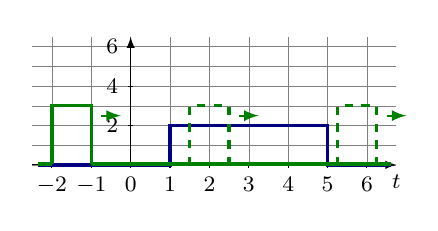
\begin{tikzpicture}
    [
    x=1cm, y=0.5cm, scale=0.5, font=\footnotesize, >=latex 
    %Voreinstellung für Pfeilspitzen
    ]
    
    %Raster im Hintergrund
    \draw[step=1, gray, very thin] (-2.5,0) grid (6.75,6.5);
    
    %Zahlen auf x-Achse
    \foreach \x in {-2,-1,0,1,2,3,4,5,6}
    \draw[shift={(\x,0)},color=black] (0pt,2pt) -- (0pt,-2pt) node[below]
    {\footnotesize $\x$};
    
    %Länge x Achse
    \draw [-latex] (-2.5,0) -- ++(9.25,0) node[below] {$t$};
    
    %Länge y Achse
    \draw [-latex] (0,0) -- ++(0,6.5) node[left] {$ $};
    
    %Zahlen auf y-Achse 
    %\foreach \y in {0,...,1}
    \foreach \y in {2,4,6}
    \draw[shift={(0,\y)},color=black] (2pt,0pt) -- (-2pt,0pt) node[left]
    {\footnotesize $\y$};		
    
    %f(t)
    \draw[blue!50!black, very thick] (-2.35,0) -- (1,0) -- (1,2) -- (5,2) -- (5,0) -- (6.6,0); 
    
    %g(t)
    \draw[green!50!black, very thick] (-2,0.05) -- (-2,3) -- (-1,3) -- (-1,0.05); 
    \draw[-latex,green!50!black, thick] (-0.75,2.5) -- (-0.25,2.5);
    
    \draw[green!50!black, very thick] (-2.35,0.05) -- (-2,0.05); 
    \draw[green!50!black, very thick] (-1,0.05) -- (6.6,0.05);		
    
    \draw[dashed, green!50!black, very thick] (1.5,0) -- (1.5,3) -- (2.5,3) -- (2.5,0); 
    \draw[-latex,green!50!black, thick] (2.75,2.5) -- (3.25,2.5);
    
    \draw[dashed, green!50!black, very thick] (5.25,0) -- (5.25,3) -- (6.25,3) -- (6.25,0); 
    \draw[-latex,green!50!black, thick] (6.5,2.5) -- (7,2.5);		
        
    
    %Vektor a
    %\draw[-latex, thick] (0,0) -- (2,3) node [midway, above] {$\vec{a}$} node (a) {}; 
    %Vektor b
    %\draw[-latex, thick] (0,0) -- (3,0) node [midway, above] {$\vec{b}$} node (b) {}; 
    %\draw[dashed] (a.center) -- ++ (3,0) node (c) {};
    %\draw[dashed] (b.center) -- ++ (2,3);
    %\draw[very thick, red, -latex] (0,0) -- (c.center) node [midway, above] {$\vec{c}$};
\end{tikzpicture}